\message{ !name(presentation.tex)}\documentclass[10pt]{beamer}
\usetheme{Antibes}

\usepackage{graphicx}
\graphicspath{{../figures/}}


\title{Gendered Pronoun Resolution}
\author[Dhruv, Prateek]{ Dhruv Patel (14528) \and Prateek Sachan (15754)}
\institute[CSA, IISc.]{Computer Science and Automation, Indian Institute of Science}
\begin{document}

\message{ !name(presentation.tex) !offset(-3) }

\begin{frame}
  \maketitle
\end{frame}

\section{Problem Introduction}
\begin{frame}{Problem}
  \begin{itemize}
  \item<+-> We are given a sentence or sentences, two candidate nouns within a sentence and a pronoun
  \item<+-> Task is to identify which of the two candidates referes to that pronoun
  \item<+-> Introduced as Kaggle competition by Google AI
  \end{itemize}

    \begin{block}<+->{Example}
      Impressed by her beauty, her warrior skills, and the fact that she was able to locate him, she is promoted to a position similar to that later held by her half-sister, Talia. As a right hand associate, she accompanies him during his adventures. Ra's is so impressed with her abilities, he even allows Nyssa to use his Lazarus Pits. Like \textit{\textbf{her}} sister \textbf{Talia}, \textbf{\underline{Nyssa}} eventually becomes disenchanted with Ra's genocidal plans to ``cleanse the Earth'', and disassociates herself from her father sometime in the early 20th century.
    \end{block}

\end{frame}

\section{Datasets}
\begin{frame}{Datasets}
  \pause
  \begin{block}<+->{GAP Webster et al. (2018)\cite{webster2018gap}}
    \begin{itemize}
    \item<+-> Balanced Dataset
    \item<+-> 2000 Development, 2000 Test and 454 validation sentences
    \end{itemize}

    \begin{quote}<+->
      \textbf{\underline{Kathleen}} first appears when \textbf{Theresa} visits \textbf{\textit{her}} in a prison in London.
    \end{quote}
  \end{block}

  \begin{block}<+->{Definite Pronoun Resoluiton, Rahman et al. (2012), \cite{rahman2012resolving}}
    \begin{itemize}
    \item<+-> Unbalanced dataset
    \item<+-> 1886 senteces in total (943 sentence pairs) (When used, we used all for training)
    \end{itemize}

    \begin{quote}<+->
       James asked \textbf{Robert} for a favor, but \textit{\textbf{he}} refused.

       \textbf{James} asked Robert for a favor, but \textit{\textbf{he}} was refused.
      
    \end{quote}
  \end{block}

\end{frame}

\subsection{Data Augmentation}
\begin{frame}{Data Augmentation}
  \begin{itemize}
  \item<+-> 2000 senteces, two less data to train.
  \item<+-> Our models quickly overfitted. We were unable to pass our own baseline.
  \end{itemize}
  \begin{block}<+->{Hypothesis}
    To neural network, if only ``Jon Snow doesn't know anything'' is given, the effect should be similar to when ``John Wick doesn't know anything'' is given instead.
  \end{block}
  
  \uncover<+->{So we replace all occurances of Jon with John and of Snow with Wick. There could be same occurance for different \textbf{unrelated} people by chance. We assume that, that doens't happen often.}

  \uncover<+->{As a side effect Ramsey Snow will become Ramsey Wick. In most cases this is not a problem. }

\end{frame}

\begin{frame}<0>{Method}
  \begin{itemize}
  \item If both candidate A and candidate B has less than four words and neither of them contains characters from ``,(*)''
    \begin{itemize}
    \item If pronoun is 
    \end{itemize}
  \end{itemize}
\end{frame}

\begin{frame}{Example}
  \begin{itemize}
  \item Tony Markham, a high school senior and the ``Tall Dark Stranger'' \underline{Betsy} fell in love with as a freshman, who has since become a good friend not only to \underline{Betsy} but the entire \underline{Ray} family. \underline{Mrs. Ray}, \underline{Betsy}'s mother. \underline{Mr. Ray}, \underline{Betsy}'s father, who owns a shoestore. \textbf{\underline{Margaret Ray}}, \textbf{\underline{Betsy}}'s sister who is five years younger than she is.
  
  \item Tony Markham, a high school senior and the ``Tall Dark Stranger'' \underline{Booth} fell in love with as a freshman, who has since become a good friend not only to \underline{Booth} but the entire \underline{Delgado} family. \underline{Mrs. Delgado}, \underline{Booth}'s mother. \underline{Mr. Delgado}, \underline{Booth}'s father, who owns a shoestore. \underline{Pam Delgado}, \underline{Booth}'s sister who is five years younger than she is.

  \item Tony Markham, a high school senior and the ``Tall Dark Stranger'' \underline{Alyssa} fell in love with as a freshman, who has since become a good friend not only to \underline{Alyssa} but the entire \underline{Jolie} family. \underline{Mrs. Jolie}, \underline{Alyssa}'s mother. \underline{Mr. Jolie}, \underline{Alyssa}'s father, who owns a shoestore. \underline{Angelina Jolie}, \underline{Alyssa}'s sister who is five years younger than she is.
  \end{itemize}    

\end{frame}

\begin{frame}
  \begin{figure}
    \centering
    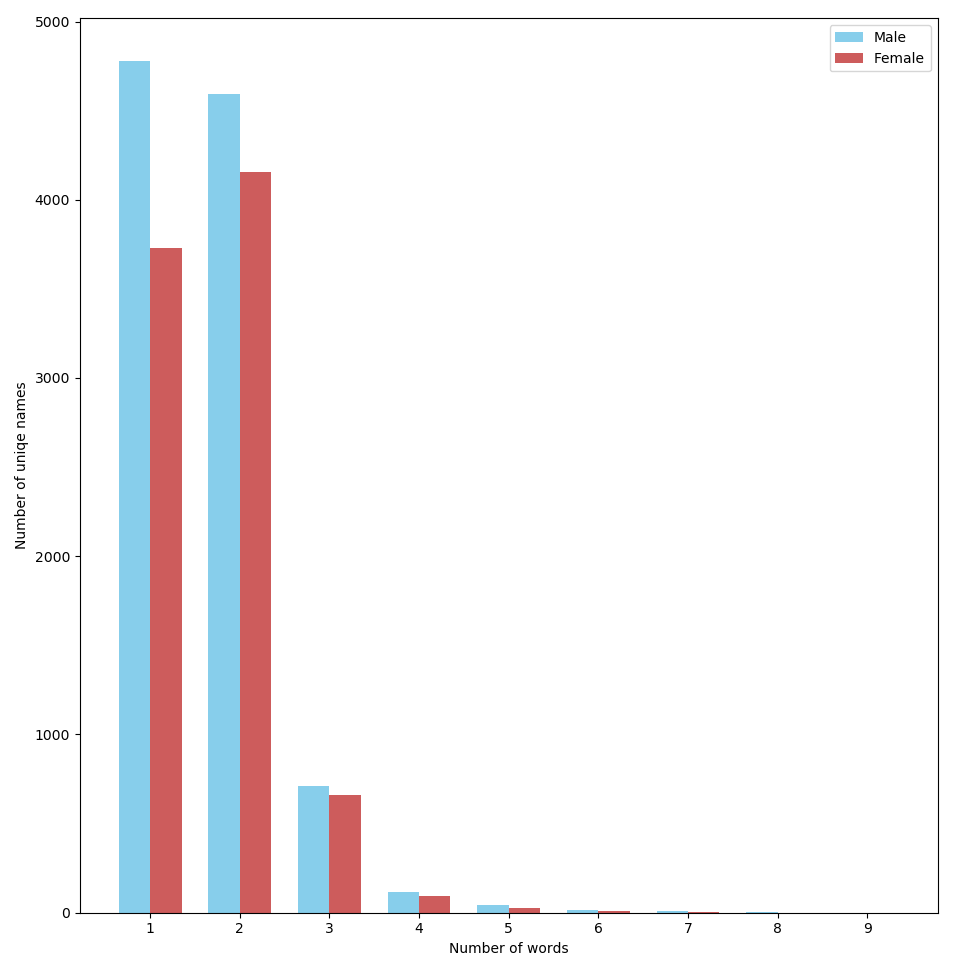
\includegraphics[width=.7\textwidth]{augment_dist.png}
    \caption{Distribution of names}
    \label{fig:dist_names}
  \end{figure}
\end{frame}

\section{}
\begin{frame}
  \frametitle{References}
  \bibliographystyle{ieeetr}
  \bibliography{presentation.bib}
\end{frame}

\end{document}
\message{ !name(presentation.tex) !offset(-116) }
